\documentclass[../Design.tex]{subfiles}

\begin{document}
    \begin{figure}[hbt!]
        \centerline{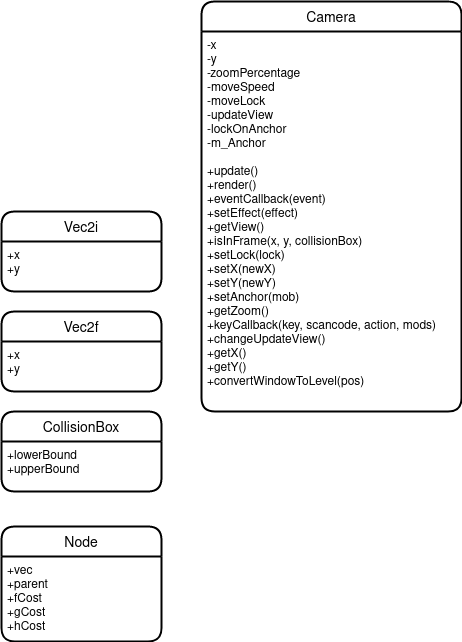
\includegraphics[scale=0.5]{img/Classes/Other.png}}
        \caption{Classes that are for general use}
        \label{fig}
    \end{figure}
    Camera
    \begin{center}
        Variables
        \begin{tabular}{ | m{0.45\textwidth} | m{0.45\textwidth} | }
            \hline
            \textbf{Variable Name} & \textbf{Description} \\
            \hline
            x & Stores x position of the camera \\
            \hline
            y & Stores the y position of the camera \\
            \hline
            zoomPercentage & Stores the zoom percentage of the objects \\
            \hline
            moveSpeed & Stores the speed it can move when disconnected from its anchor \\
            \hline
            moveLock & Stores whether it can move or not \\
            \hline
            updateView & Stores whether the view effect needs to be updated \\
            \hline
            lockOnAnchor & Stores whether it needs to be locked on its anchor \\
            \hline
            m\_Anchor & Stores the entity it is locked onto \\
            \hline
        \end{tabular}
        Functions
        \begin{tabular}{ | m{0.2\textwidth} | m{0.3\textwidth}| m{0.4\textwidth} | }
            \hline
            \textbf{Function Name} & \textbf{Parameters} & \textbf{Description} \\
            \hline
            update & & Updates the camera position \\
            \hline
            render & & Updates the view effect \\
            \hline
            eventCallback & event & Deals with current event \\
            \hline
            setEffect & effect & Allows camera to receive an effect \\
            \hline
            getView & & Returns the view matrix \\
            \hline
            isInFrame & Position and collision box & Returns whether it will be displayed onscreen \\
            \hline
            setLock & lock & Sets the lock \\
            \hline
            setX & new x coord & sets the x value \\
            \hline
            setY & new y coord & sets the y value \\
            \hline
            setAnchor & mob & Sets the anchor  \\
            \hline
            getZoom & & Returns the zoom \\
            \hline
            keyCallback & information stored in key event & Deals with a key being pressed \\
            \hline
            changeUpdateView & & changes the updateView variable to true so the view will be updated next render cycle \\
            \hline
            getX & & Returns the x value \\
            \hline
            getY & & Returns the y value \\
            \hline
            convertWindowToLevel & Position vector & Converts the position into coordinates in the level \\
            \hline
        \end{tabular}
    \end{center}
    Vec2i
    \begin{center}
        Variables
        \begin{tabular}{ | m{0.45\textwidth} | m{0.45\textwidth} | }
            \hline
            \textbf{Variable Name} & \textbf{Description} \\
            \hline
            x & Stores x position as an int \\
            \hline
            y & Stores y position as an int \\
            \hline
        \end{tabular}
    \end{center}
    Vec2f
    \begin{center}
        Variables
        \begin{tabular}{ | m{0.45\textwidth} | m{0.45\textwidth} | }
            \hline
            \textbf{Variable Name} & \textbf{Description} \\
            \hline
            x & Stores x position as an float \\
            \hline
            y & Stores y position as an float \\
            \hline
        \end{tabular}
    \end{center}
    CollisionBox
    \begin{center}
        Variables
        \begin{tabular}{ | m{0.45\textwidth} | m{0.45\textwidth} | }
            \hline
            \textbf{Variable Name} & \textbf{Description} \\
            \hline
            lowerBound & Stores the position of the bottom left corner (relative to the objects coordinates) \\
            \hline
            upperBound & Stores the position of the top right corner (relative to the objects coordinates) \\
            \hline
        \end{tabular}
    \end{center}
    Node
    \begin{center}
        Variables
        \begin{tabular}{ | m{0.45\textwidth} | m{0.45\textwidth} | }
            \hline
            \textbf{Variable Name} & \textbf{Description} \\
            \hline
            vec & Stores the position of the node (as integer in the grid) \\
            \hline
            parent & Stores the parent (as a position on the grid) \\
            \hline
            fCost & The total cost of the node \\
            \hline
            gCost & The distance from the start node \\
            \hline
            hCost & The distance from the destination node \\
            \hline
        \end{tabular}
    \end{center}
\end{document}